% @HEADER
% ***********************************************************************
% 
%            Trilinos: An Object-Oriented Solver Framework
%                 Copyright (2001) Sandia Corporation
% 
% Under terms of Contract DE-AC04-94AL85000, there is a non-exclusive
% license for use of this work by or on behalf of the U.S. Government.
% 
% This library is free software; you can redistribute it and/or modify
% it under the terms of the GNU Lesser General Public License as
% published by the Free Software Foundation; either version 2.1 of the
% License, or (at your option) any later version.
%  
% This library is distributed in the hope that it will be useful, but
% WITHOUT ANY WARRANTY; without even the implied warranty of
% MERCHANTABILITY or FITNESS FOR A PARTICULAR PURPOSE.  See the GNU
% Lesser General Public License for more details.
%  
% You should have received a copy of the GNU Lesser General Public
% License along with this library; if not, write to the Free Software
% Foundation, Inc., 59 Temple Place, Suite 330, Boston, MA 02111-1307
% USA
% Questions? Contact Michael A. Heroux (maherou@sandia.gov) 
% 
% ***********************************************************************
% @HEADER

\documentclass[10pt,relax]{SANDreport}
\usepackage{amsmath,amsthm}
\usepackage{amssymb}
\usepackage{amsfonts}
\usepackage{palatino}
\usepackage{rotating,tabularx}

\def\choicebox#1#2{\noindent$\hphantom{th}$\parbox[t]{1.8in}{\sf
#1}\parbox[t]{4.5in}{#2}\\[0.8em]}

\author{Marzio Sala, Micheal Heroux\\
Computational Mathematics and Algorithms Department \\ [10pt]
William F. Spotz, Eric T. Phipps \\
Applied Computational Methods Department \\ [10pt]
Sandia National Laboratories \\
P.O. Box 5800 \\
Albuquerque, NM 87185-1110 \\
}

\title{An Overview of PyTrilinos}
\SANDnum{SAND2005-XXXX}
\SANDauthor{
Marzio Sala, William F. Spotz, Eric T. Phipps, Micheal A. Heroux}

\SANDprintDate{June 2005}
\SANDreleaseType{Unlimited Release}

\newcommand{\PyTrilinos}{{PyTrilinos}}
\newcommand{\Trilinos}{{Trilinos}}
\newcommand{\TrilinosTM}{Trilinos \copyright}
\newcommand{\trilinos}{{Trilinos}}
\newcommand{\ifpack}{{Ifpack}}
\newcommand{\aztecoo}{{AztecOO}}
\newcommand{\amesos}{{Amesos}}
\newcommand{\epetra}{{Epetra}}
\newcommand{\ml}{{ML}}
\newcommand{\mb}[1]{{\mathbf {#1} }}
\newcommand{\teuchos}{{Teuchos}}
\newcommand{\triutils}{{Triutils}}
\newcommand{\metis}{{METIS}}

\newcommand{\ie}{i.e., }
\newtheorem{assumption}{Assumption}[section]
\newtheorem{lemma}{Lemma}[section]
\newtheorem{proposition}{Proposition}[section]
\newtheorem{corollary}{Corollary}[section]
\newtheorem{theorem}{Theorem}[section]
\newtheorem{algorithm}{Algorithm}[section]
\newtheorem{definition}{Definition}[section]
\newtheorem{property}{Property}[section]
\newtheorem{interface}{Interface}[section]
\newtheorem{remark}{Remark}
\newcommand{\note}[1]{\begin{center}\fbox{\bf #1}\end{center}}


\def\choicebox#1#2{\noindent$\hphantom{th}$\parbox[t]{3.0in}{\sf
#1}\parbox[t]{3.35in}{#2}\\[0.8em]}

\begin{document}

\maketitle

\begin{abstract}
\PyTrilinos\ is a collection of Python modules that are useful for
serial and parallel scientific computing. This collection contains
modules that cover serial dense linear algebra, parallel sparse linear
algebra, direct and iterative linear solution techniques, domain
decomposition and multilevel preconditioners, nonlinear solvers and
continuation algorithms. Also included are a variety of related
utility functions and classes, including distributed I/O and matrix generation
utilities.
\PyTrilinos\ vector objects are integrated with the popular Numeric
Python module, gathering together a variety of high-level distributed
computing with serial vector operations.

PyTrilinos is defined as a set of interfaces to already available non-Python
libraries.
This hybrid framework uses Python as front-end, and
efficient precompiled libraries for all computationally expensive tasks. Thus,
we take advantage of both the flexibility and ease of use of Python,
and the efficiency of the underlying C++, C and FORTRAN numerical
kernels.

To run in parallel, \PyTrilinos\ simply requires a standard Python
interpreter.  The fundamental MPI calls are abstracted beneath the
Epetra module layer, and all inter-processor communications by all
\PyTrilinos\ modules are handled using Epetra communicators. This
makes serial and parallel scripts using \PyTrilinos\ virtually
identical.
\end{abstract}

\clearpage
\section*{Acknowledgments}
The authors would like to acknowledge the support of the ASCI and LDRD
programs that funded development of Trilinos, and all the Trilinos
developers for their contribution to Trilinos, without which
\PyTrilinos\ would not exist.

\medskip

\SANDmain
\tableofcontents
\newpage

%-----------------------------------------------------------------------------
\section{Introduction}
\label{sec:intro}
%-----------------------------------------------------------------------------

The choice of the programming language for the development and usage of
large-scale, high-performance numerical algorithm is often a thorny issue.
Ideally, the programming language is only a tool used to produce a working
library or application. In practice, the are important differences between the
several programming languages made available to developers---from FORTRAN77 or
FORTRAN90, to C and C++, Java, Python, and several others. An important
distinction can be made between {\sl interpreted} languages and {\sl compiled}
languages. For the former, the list of instructions (called {\sl script}) is
translated at run-time by an interpreter, then executed; for the latter, the
code is compiled and an executable is created. It is well known that
interpreted code is easier to use and debug as the interpreter will analyze each
instruction as it is executed. This comes at a computational price, since the interpreter
may require several CPU cycles to parse each instruction. Therefore,
interpreted languages are usually disregarded by developers of
high-performance applications (often as a pre-conceptual idea). Almost all
high-performance libraries are written in compiled languages
such as C, C++ or FORTRAN. Using these languages, developers can obtain 
high performance and portable codes,
since these languages are reasonably well standarized and compilers quite
mature on almost all platforms.  However,
these languages require constant attention to low-level system
programming, like memory allocation and deallocation.  Because
compilation and linking are essential steps, the development cycle can
be slowed down considerably.  

Our interest is in a high-level, flexible programming environment,
with performance comparable to that of native C, C++ or FORTRAN
code. Flexibility is fundamental to allow rapid prototyping, in the
sense that the developer should be able to write a basic code
satisfying his or her needs in a very short time.  However, it is
almost impossible for a single programming language to be at the same
time easy-to-use, allow fast development, and produce optimized
executables. Indeed, the goals of efficiency and flexibility are often
in conflict with each other.

From our point of view, the key observation is that, for most
applications, the time-critical portion of the code that requires the
efficiency of a compiled language is related to a small set of
self-contained functions or classes. Therefore, one can adopt an
interpreted (and possibly interactive) language, without a big
performance degradation, provided there is a robust interface between
the interpreted and compiled languages. Among the available scripting
languages, we decided to adopt Python. Python
is an interpreted, interactive, object-oriented programming
language, which combines remarkable power with very clean syntax (it
is often observed that well-written Python code reads like pseudo
code).  Perhaps most importantly, it can be easily extended using
modules written in C or C++ for all performance critical tasks.

This article describes a collection of numerical analysis algorithms, called
PyTrilinos, 
built on top of the Trilinos
project~\cite{Trilinos-home-page,Heroux:2005:OTP}.  It adds significant power
to the interactive Python session by exposing the user to high-level commands
and classes for the creation, handling and usage of serial dense and
distributed sparse linear algebra objects. Using \PyTrilinos, an interactive
Python session becomes a powerful data-processing and system-prototyping
environment that can be used to test, validate, use
and extend serial and parallel numerical algorithms.
In our opinion, Python naturally complements
system languages like C, C++ and FORTRAN rather than competing with
them.

%Python is a high-level general purpose programming language. Because
%code is automatically compiled to byte code and executed, Python is
%suitable for use as a scripting language.  In typical Python
%development, a system's frontend and infrastacture may be written in
%Python for ease of development and modification, but the kernel is
%still written in C or C++ for efficiency.  We use Python as a glue
%between different modules, written in high-performance languages; each
%of these modules is an already available library, dynamically loaded
%by Python when required.  

\smallskip

This document is organized as follows. Section~\ref{sec:design} describes the
project design, the organization of PyTrilinos and its division into modules.
Comments on the usage of
parallel, MPI Python scripts using PyTrilinos are reported in
Section~\ref{sec:serial}. Examples of usage and comparisons between Trilinos
and PyTrilinos codes are reported in Section~\ref{sec:comparision}.
Section~\ref{sec:related} positions PyTrilinos with respect to similar
projects. COncluding remarks are reported in Section~\ref{sec:concluding}.

%-----------------------------------------------------------------------------
\section{Project Design}
\label{sec:design}
%-----------------------------------------------------------------------------

%-----------------------------------------------------------------------------
\subsection{Why Python}
\label{sec:why}
%-----------------------------------------------------------------------------

Python has emerged as an excellent choice for scientific computing
because of its simple syntax, ease of use, and elegant
multi-dimensional array arithmetic. Its interpreted evaluation allows
it to serve as both the development language and the command line
environment in which to explore data. Python also excels as a ``glue''
language between a large and diverse collection of software packages
-- a common need in the scientific arena.

Python combines remarkable power with very clean syntax. It has
modules, classes, exceptions, high-level dynamic data types, automatic
memory management that frees the user from most hassles of memory
allocation, and much more. Python also has some features that make it
possible to write large programs, even though it lacks most forms of
compile-time checking: a program can be constructed out of modules,
each of which defines its own namespace. Exception handling makes it
possible to catch errors where required without cluttering the code
with error checking.

Python's development cycle is dramatically shorter than that of
traditional tools. In Python, there are no compile or link
steps--Python programs simply import modules at runtime and use the
objects they contain. Because of this, Python programs run immediately
after changes are made. Python integration tools make it usable in
hybrid, multi-compont applications. As one consequence, systems can
simultaneously utilize the strengths of Python for rapid development,
and of traditional languages such as C for rapid execution.  This
flexibility of development modes is crucial in realistic environments.
Python is optimized for speed of development, but that alone is not
enough.

\note{Why no other scripting languages?}

%-----------------------------------------------------------------------------
\subsection{Multilevel Organization of PyTrilinos}
\label{sec:multilevel}
%-----------------------------------------------------------------------------
  
\PyTrilinos\ is a designed as a modular multilevel framework, and it
takes advantage of several programming languages at different levels.
The key components are:
\begin{enumerate}

\item {\bf Trilinos}, a set of numerical solver packages in active
  development that allows high-performance scalable linear algebra
  operations for problems defined on sparse matrices. Trilinos
  contains more that half a million of code lines, and it can
  interface to several third-party libraries. The source codes of the
  ``stable'' linear algebra packages of Trilinos account for about 300,000
  code lines, divided in about 67,000 code lines for distributed linear
  algebra objects and utilities, 20,000 code lines for direct solvers and
  interfaces to third-party direct solvers, 128,000 code lines for multilevel
  preconditioners, and 76,000 code lines for other algebraic preconditioners
  and Krylov accelerators.

\item {\bf Numeric}, a well-established Python module to handle
  matrices and vectors; see~\cite{numeric}.

\item {\bf SWIG}, the Simplified Wrapper and Interface Generator,
  which is a preprocessor that turns ANSI C/C++ declarations into
  scripting language interfaces, and produces a fully working Python
  extension module; see~\cite{swig}.

\item {\bf Distutils}, a Python module with utilities aimed at the
  portable distribution of both pure Python modules and compiled
  extension modules.  Distutils has been a part of the standard Python
  distribution since Python version 2.2.

\end{enumerate}

A description of the organization of  the linear algebra modules of
PyTrilinos, with some of the third-party libraries can be accessed,
is reported in Figure~\ref{fig:organization}.

\begin{figure}
\begin{center}
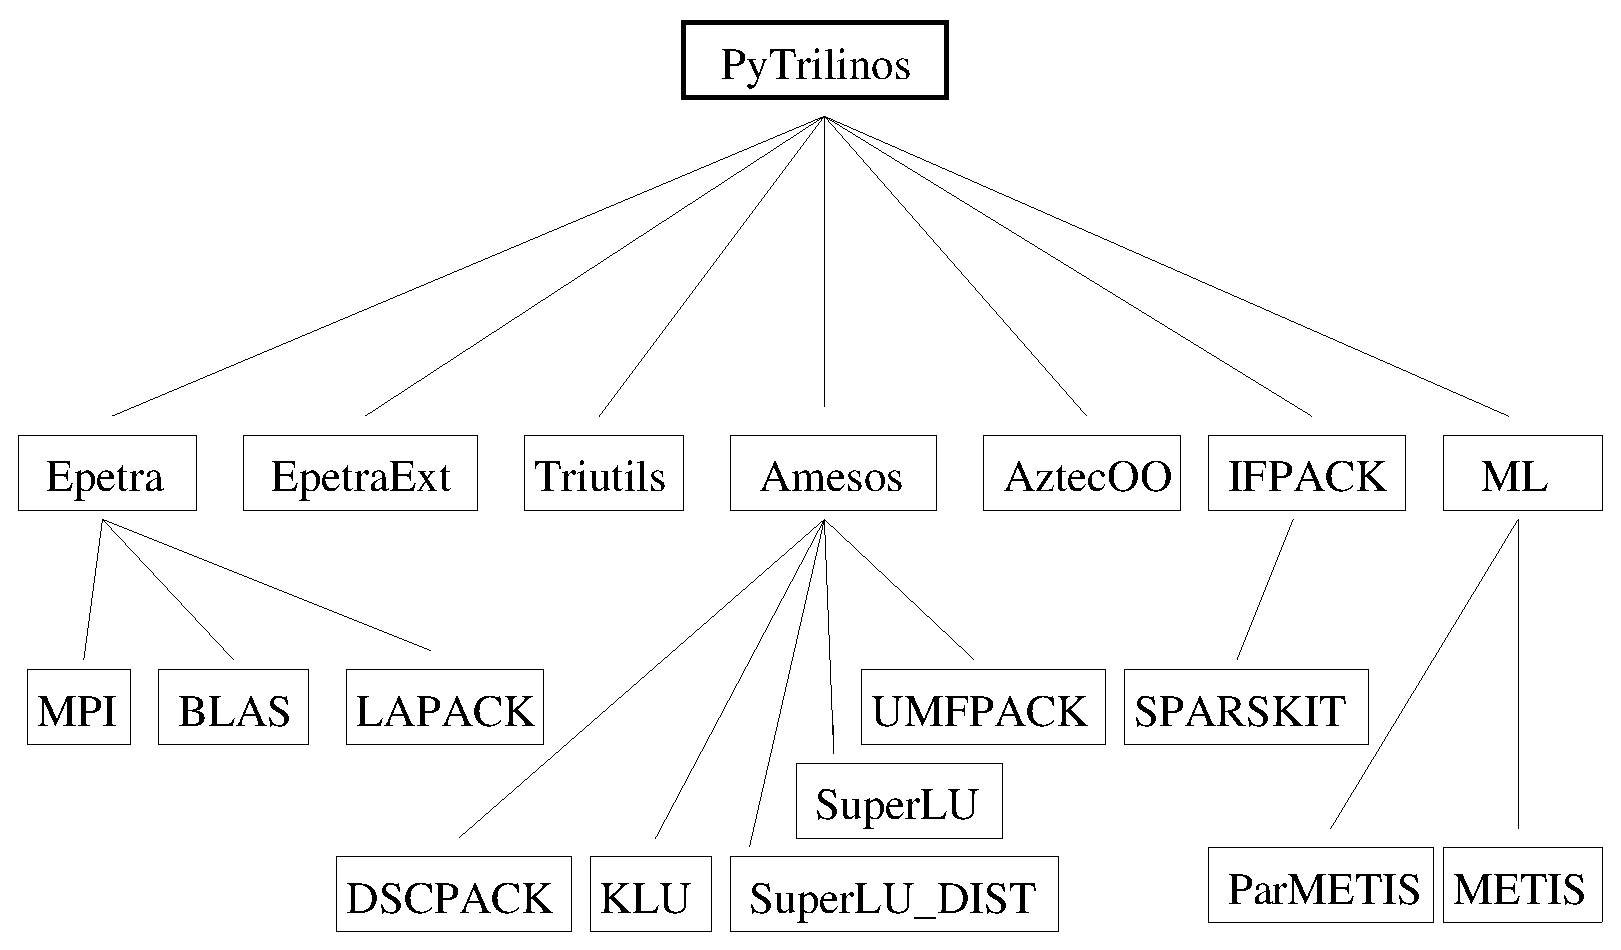
\includegraphics[width=12cm]{../UsersGuide/organization.eps}
\caption{Organization of the linear algebra modules of PyTrilinos.}
\label{fig:organization}
\end{center}
\end{figure}

%-----------------------------------------------------------------------------
\subsection{PyTrilinos Organization}
\label{sec:organization}
%-----------------------------------------------------------------------------

\PyTrilinos\ reflects the Trilinos organization by presenting a series
of {\sl modules}, each of them wraps a given Trilinos {\sl package},
 where a package is an integral unit usually
developed by a small team of experts in a particular area.
Trilinos packages that support namespaces have a Python submodule for
each namespace.  Algorithmic capabilities are defined within
independent packages. The modules of \PyTrilinos\ are:

\begin{enumerate}

\item {\bf Epetra}, a collection of concrete classes to support the
  construction and use of vectors, sparse graphs, and dense and sparse
  matrices. It provides serial, parallel and distributed memory
  capabilities. Two Epetra objects are important for this
  discussion. The first object is a {\sl communicator}, which
  encapsulates all the inter-processor data exchange. The second
  object is a {\sl map}, which describes the domain decomposition of
  distributed linear algebra objects. Serial runs make use of trivial
  communicators and maps; parallel runs adopt an MPI-based
  communicator and support arbitrary maps. See~\cite{epetra-guide} for
  more details.  Epetra uses BLAS and LAPACK where possible, and as a
  result has good performance characteristics.

\item {\bf EpetraExt} offers a variety of extension capabilities to
  the Epetra package, such as input/output and coloring algorithms.
  The I/O capabilities make it possible to read and write generic
  Epetra objects (like maps, matrices and vectors).

\item {\bf Triutils} allows the creation of several matrices, like the
  MATLAB's {\tt gallery} function, and it can be useful for examples
  and testing. Some input capabilities make it possible to read a matrix in
  Harwell/Boeing or MatrixMarket format, therefore accessing a large variety
  of well-recognized test cases for dense and sparse linear algebra.

\item {\bf Amesos} contains a set of clear and consistent interfaces
  to the following third-party serial and parallel sparse direct
  solvers: UMFPACK~\cite{umfpack-acm-toms},
  PARDISO~\cite{pardiso-manual}, TAUCS~\cite{taucs-home-page}, SuperLU
  and SuperLU\_DIST~\cite{superlu-manual},
  DSCPACK~\cite{dscpack-manual}, and MUMPS~\cite{mumps-manual}. As
  such, \PyTrilinos\ makes it possible to access state-of-the-art
  direct solver algorithms developed by groups of specialists, and
  written in different languages (C, FORTRAN77, FORTRAN90), in both
  serial and parallel. By using Amesos, more than 350,000 code lines (without
  considering BLAS, LAPACK, and ScaLAPACK) can be easily accessed from any
  code based on Trilinos (and therefore PyTrilinos).  We refer to the Amesos
  reference guide~\cite{Amesos-Reference-Guide} for more details.

\item {\bf AztecOO} contains preconditioned Krylov accelerators, like
  CG, GMRES and several others~\cite{golub96matrix}, based on the popular Aztec
  library~\cite{aztecoo-guide}.  One-level domain decomposition
  preconditioners based on incomplete factorizations are available.

\item {\bf IFPACK} contains object-oriented algebraic preconditioners,
  compatible with Epetra and AztecOO.  It supports construction and
  use of parallel distributed memory preconditioners such as
  overlapping Schwarz domain decomposition with several local solvers.
  IFPACK can take advantage of SPARSKIT~\cite{sparskit}, a venerable
  but successful software package; see~\cite{ifpack-guide}.

\item {\bf ML} contains a set of multilevel preconditioners based on
  aggregation procedures for serial and vector problems compatible with Epetra
  and AztecOO. ML can take
  advantage of the METIS~\cite{metis} ParMETIS~\cite{parmetis}
  libraries to create the aggregates.  For a general introduction to
  ML and its applications, we refer to the ML Users
  Guide~\cite{ml-guide}.

\end{enumerate}

Note that all third-party libraries (except BLAS and LAPACK) are
optional and do not need to be installed to use \PyTrilinos\ (or
Trilinos).

\note{Say something about modularity, users may decide to compile and/or use
  only some of the packages}

Epetra is the ``language'' of Trilinos, and offers a convenient set of
interfaces to define distributed linear algebra objects. Epetra
supports double-precision floating point data only (no
single-precision or complex).  \PyTrilinos\ cannot be used without the
Epetra module.

%-----------------------------------------------------------------------------
\section{Serial and Parallel Environments}
\label{sec:serial}
%-----------------------------------------------------------------------------

Although testing and development of high-performance algorithms can be done in
serial environments, parallel environments still constitute the most
important field of application for most of Trilinos' algorithms. However,
  Python itself does not provide any parallel support. Because of this reason,
  several projects entered the scene, to fulfill the gap between Python and
  MPI applications. We have analyzed the following:
\begin{itemize}
\item {\bf MPI Python (pyMPI)} is a framework for developing parallel Python
  applications using MPI~\cite{MPI-Python};
\item {\bf PyPAR} is a more light-weight wrapper of the MPI library
  for Python~\cite{pypar}.
\item {\bf Python BSP} supports the more high-level Bulk Synchronous
  Parallel approach~\cite{FIXME}
\end{itemize}

All these projects allow the use of Python through the interactive  prompt, 
  but an additional overhead is introduced. Besides, none of these projects
  defines a well-recognized standard, since they are still under heavy
  development. 

Our approach is somehow complementary to the efforts of these projects. 
We decided to use a standard, out-of-the-box, Python interpreter, then wrap all MPI calls
through the Epetra package. In fact, all wrapped Trilinos packages are already
based on Epetra communicators. This reflects the philosophy of all the
considered
Trilinos packages, that have no explicit dependency on MPI communicators, and
accept the pure virtual class Epetra\_Comm instead. PyTrilinos scripts create
a communicator using command
\begin{verbatim}
    comm = Epetra.PyComm()
\end{verbatim}
which returns an {\tt Epetra.SerialComm} if \PyTrilinos\ has been compiled
in serial mode, or an {\tt Epetra.MpiComm} if \PyTrilinos\ has support for
MPI. By using {\tt Epetra.PyComm}, \PyTrilinos\ scripts are virtually
identical for both serial and parallel runs, and generally reads:
\begin{verbatim}
    >>> from PyTrilios import Epetra
    >>> Epetra.Init()
    >>> comm = Epetra.PyComm()
        ...
    >>> Epetra.Finalize()
\end{verbatim}
A pictorial representation of how communication are handled in
the case of two  processors is given in Figure~\ref{fig:distributed}. For
serial runs, both Init() and Finalize() are empty instructions.

\smallskip

The major disadvantage of this approach is that Python cannot be run
interactively if more than one processor is used, and we experienced problems
with some MPI interpreters (in particular MPICH) to execute Python scripts.
Besides, although all the most important MPI calls are available through
Epetra.Comm objects (for example, the rank of a process is returned by method
                     {\tt Comm.MyPID()} and the number of processes involed in
                     the computation by method {\tt Comm.NumProc()}), not all
the functions specified by the MPI forum are readily available through the
Comm object.  For example, there are no point-to-point communications, or
non-blocking functions. Also, PyTrilinos always uses MPI\_COMM\_WORLD as basic
communicator.

In our opinion, these are only minor drawbacks, and the list
of advantages is much longer. 
First, since all
calls are handled by Epetra, no major overhead occurs, other than that of
parsing a Python instruction. Second, all PyTrilinos modules that require
direct MPI calls can dynamic cast the Epetra.Comm object, retrive the MPI
communicator object, then use direct C/C++ MPI calls. As such, the entire set of MPI
function is available to developers. Third, a standard Python interpreter is
required. Finally, serial and paralle scripts are identical, and 
 PyTrilinos scripts can be run in parallel
by using an instruction of type
\begin{verbatim}
    % mpirun -np 4 python ./my-script.py
\end{verbatim}
where {\tt my-script.py} contains at least the basic instructions required
to define an Epetra.PyComm.

\begin{figure}
\begin{center}
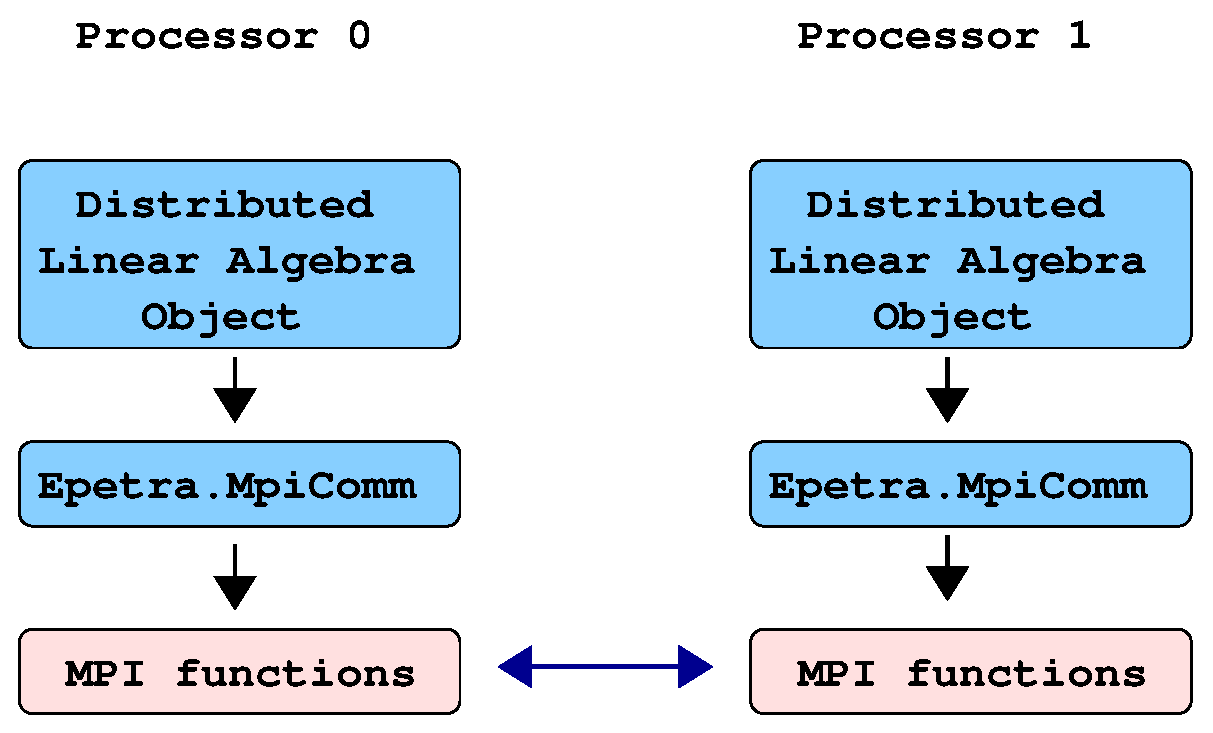
\includegraphics[height=5cm]{../UsersGuide/distributed_object.eps}
\caption{All distributed PyTrilinos objects are based on the Epetra.MpiComm
  object, which takes care of calling MPI functions for intra-processor
    communications.}
\label{fig:distributed}
\end{center}
\end{figure}


%-----------------------------------------------------------------------------
\section{Using PyTrilinos}
\label{sec:using}
%-----------------------------------------------------------------------------

In order to present the functionalities of PyTrilinos, this Section will
briefly describe the main capabilities of all modules, together with a brief
mathematical background of the implemented algorithms.

%-----------------------------------------------------------------------------
\subsection{The Epetra Module}
\label{subsec:epetra}
%-----------------------------------------------------------------------------

Epetra provides an extensive set of classes to create and fill
distributed sparse matrices. These classes allow row-by-row or
element-by-element constructions. Support is provided for common
matrix operations, including scaling, norm, matrix-vector
multiplication and matrix-multivector multiplication.  Using Epetra
objects, applications do not need to know about the particular storage
format, and other implementation details such as data layout, the
number and location of ghost nodes. Matrices can be stored row-by-row using
class Epetra.CrsMatrix, and vectors with classes Epetra.Vector and
Epetra.MultiVector.
Another useful class is Epetra.FECrsMatrix.  The most important
additional feature provided by the Epetra.FECrsMatrix compared
to Epetra.CrsMatrix, is the capability to set non-local matrix
elements. Serial dense linear algebra is supported 
(as a light-weight on the top of BLAS and LAPACK) through classes
Epetra.SerialDenseVector and Epetra.SerialDenseMatrix.
 Class Epetra.Time can be used
to track the elapsed CPU time, and class Epetra.CrsGraph to define distributed
graphs.

%-----------------------------------------------------------------------------
\subsection{The Triutils Module}
\label{subsec:triutils}
%-----------------------------------------------------------------------------

Triutils provides matrix reading and matrix generation capabilities. This
module is mainly meant for testing solvers. A function is available to read a
matrix from the popular Harwell/Boeing format.
Several matrices, corresponding to finite difference discretization of model
problems, can be generated using the matrix gallery of Triutils, which
provides functionalities similar to that of the MATLAB's {\tt gallery}
command; see~\cite[Chapter 5]{Trilinos-tutorial} for more details.

%-----------------------------------------------------------------------------
\subsection{The Amesos Module}
\label{subsec:amesos}
%-----------------------------------------------------------------------------

Once a (square) sparse matrix and two vectors are created, an
important problem is how to solve the corresponding linear system
\begin{equation}
  \label{eq:lin_sys}
  A X = B
\end{equation}
where $A \in \mathbb{R}^{n \times n}$ is a sparse linear operator, $X
\in \mathbb{R}^{n \times m}$ and $B \in \mathbb{R}^{n \times m}$ are
the solution and right-hand side, respectively. Parameter $n$ is the
global dimension of the problem, and $m$ is the number of vectors in
the multi-vectors $X$ and $B$.  (If $m = 1$, then $X$ and $B$ are
``normal'' vectors.)  Linear systems of type (\ref{eq:lin_sys}) arise
in a variety of applications, and constitute the innermost
computational kernel, and often the most time-consuming of several
numerical algorithms. An efficient solver for Equation
(\ref{eq:lin_sys}) is of fundamental importance for most PDE solvers,
both linear and non-linear.

\smallskip

Probably, the most robust strategy to solve (\ref{eq:lin_sys})
is to factorize the linear matrix $A$ into the product of two matrices
$L$ and $U$, so that $A = L \, U$, and the linear systems with $L$ and
$U$ are readily solvable. Typically, $L$ and $U$ are a lower and upper
triangular matrix, respectively, and the process is referred to as
Gaussian elimination. In PyTrilinos, the direct solution of large linear
system is performed by the Amesos module, which defines interfaces to
third-party direct solvers.
All Amesos objects are constructed from the function class {\tt
  Amesos}.   The main goal of this class is to allow the user to select
any supported (and enabled at configuration time) direct solver,
simply changing an input parameter. An example of script reading the linear
system stored in the Harwell/Boeing format, the solving the problem using
SuperLU is reported in Figure~\ref{fig:amesos}.
Several parameters, specified using Python's dictionaries, are available to toggle the selected Amesos solver.

\begin{figure}
\begin{center}
\begin{tabular}{| p{12cm} |}
\hline
\\
\footnotesize
\begin{minipage}{11.5cm}
\begin{verbatim}
#! /usr/bin/env python
try:
  from PyTrilinos import Amesos, Triutils, Epetra
except ImportError:
  raise ImportError, "error w/ Amesos or Triutils or Epetra"

Epetra.Init()
Comm = Epetra.PyComm()
Map, Matrix, LHS, RHS, Exact = Triutils.ReadHB("fidap035.rua", Comm)

Problem = Epetra.LinearProblem(Matrix, LHS, RHS);
Factory = Amesos.Factory()
SolverType = "SuperLU"
Solver = Factory.Create(SolverType, Problem)
AmesosList = {
  "PrintTiming": True,
  "PrintStatus": True
}
Solver.SetParameters(AmesosList)
Solver.SymbolicFactorization()
Solver.NumericFactorization()
Solver.Solve()
LHS.Update(-1.0, Exact, 1.0)
norm = LHS.Norm2()
print '||x_computed - x_exact||_2 = ', norm[1]
Epetra.Finalize()
\end{verbatim}
\end{minipage}
\\
\\
\hline
\end{tabular}
\caption{Complete script that solves a linear system using Amesos/SuperLU.}
\label{fig:amesos}
\end{center}
\end{figure}

%-----------------------------------------------------------------------------
\subsection{The AztecOO and IFPACK Modules}
\label{subsec:aztecoo_ifpack}
%-----------------------------------------------------------------------------

For a sparse matrix, the major inconvenience of direct solution
methods is that the $L$ and $U$ factors are typically much denser than
the original matrix $A$, making Gaussian elimination too memory
demanding for large scale problems. Moreover, the factorization
process is inherently serial, and parallel factorization algorithms
can be successfully used only with a relatively modest number of
processors. The forward and back triangular solves typically exhibit
very poor parallel speedup.

A very well known solution to this problem is to adopt an iterative
solution process, like conjugate gradient or GMRES~\cite{golub96matrix}. The
rationale behind iterative methods is that they only require (at least
in their simplest form) matrix-vector and vector-vector products, and
both operations scale well for sparse matrices.

Unfortunately, the convergence of iterative methods is determined by
the spectral properties of the matrix $A$ (typically, its condition
number $\kappa(A)$), and for real-life problems $\kappa(A)$ is
``large'', meaning that the iterative solution method will converge
slowly. To solve this problem, the original linear system is replaced
by
\[
A P^{-1} P X = B
\]
where $P$, called a {\sl preconditioner}, is an operator whose inverse
aim to represent the inverse of $A$, though being much cheaper to
compute.  $P$ is chosen so that $AP^{-1}$ is easier to solver than $A$
(that is, it is better conditioned).

\smallskip

Often, algebraic preconditioners are adopted, that is, $P$ is
constructed by manipulating the entries of $A$. This gives rise to the
so-called incomplete factorization preconditioners (ILU) or algebraic
multilevel methods.

Because ILU preconditioners do not scale well on parallel computers, a
common practice is to perform {\em local} ILU factorizations.  In this
situation, each processor computes a factorization of a subset of
matrix rows and columns independently from all other processors.  This
additional layer of approximation leads to a block Jacobi type of
preconditioner across processors, where each block is solved using an
ILU preconditioner.  The difficulty with this type of preconditioner
is that it tends to become less robust and require more iterations as
the number of processors used increases.  This effect can be offset to
some extent by allowing {\em overlap}.  Overlap refers to having
processors redundantly own certain rows of the matrix for the ILU
factorization.  Level-1 overlap is defined so that a processor will
include rows that are part of its original set.  In addition, if row
$i$ is part of its original set and row $i$ of $A$ has a nonzero entry
in column $j$, then row $j$ will also be included in the factorization
on that processor.  Other levels of overlap are computed recursively.

What we have just described is an example of one-level overlapping
domain decomposition (DD) preconditioners.  The basic idea of DD
methods consists in dividing the computational domain into a set of
subdomains, which may or may not overlap. We will focus on overlapping
DD methods only, because they can be re-interpreted as algebraic
manipulation of the assembled matrix, thus allowing the construction
of black-box preconditioners. Overlapping DD methods are often
referred to as overlapping Schwarz methods. DD preconditioners can be
written as
\begin{equation}
  \label{eq:prec_dd}
  P^{-1} = \sum_{i=1}^M R_i^T B_i^{-1} R_i,
\end{equation}
where $M$ represents the number of subdomains, $R_i$ is a rectangular
Boolean matrix that restricts a global vector to the subspace defined
by the interior of the $i$th subdomain, and $B_i$ approximates the
inverse of
\begin{equation}
  \label{eq:aztecoo_tilde_a}
  A_i = R_i A R_i^T ,
\end{equation}
for example, being its ILU factorization.

To adopt an iterative solver (for example, CG),
with 1550 maximum iterations and a tolerance of $10^{-5}$ on the
relative residual, \PyTrilinos\ requires the instructions reported in
Figure~\ref{fig:aztecoo}. The script refines a preconditioner of type
(\ref{eq:prec_dd}), using AztecOO's factorizations to solve the local
problems. The sparsity pattern of a matrix is visualized
with the instruction \verb!PrintSparsity()! of the IFPACK module;
an example of output is reported in
Figure~\ref{fig:sparsity}. IFPACK can
also be used to define other flavors of domain decomposition preconditioners.

\begin{figure}
\begin{center}
\includegraphics[height=5cm]{../UsersGuide/sparsity.ps}
\caption{Sparsity pattern of matrix {\tt fidap05} obtained using {\tt
  IFPACK.PrintSparsity()}.}
\label{fig:sparsity}
\end{center}
\end{figure}

\begin{figure}
\begin{center}
\begin{tabular}{| p{12cm} |}
\hline
\\
\footnotesize
\begin{minipage}{11.5cm}
\begin{verbatim}
#! /usr/bin/env python
try:
  from PyTrilinos import IFPACK, AztecOO, Triutils, Epetra
except ImportError:
  raise ImportError, "error w/ IFPACK, AztecOO or Triutils or Epetra"

Epetra.Init()
Comm = Epetra.PyComm()
Map, Matrix, LHS, RHS, Exact = Triutils.ReadHB("fidap035.rua", Comm)

IFPACK.PrintSparsity(Matrix, "matrix.ps")

Solver = AztecOO.AztecOO(Matrix, LHS, RHS)
Solver.SetAztecOption(AztecOO.AZ_solver, AztecOO.AZ_cg)
Solver.SetAztecOption(AztecOO.AZ_precond, AztecOO.AZ_dom_decomp)
Solver.SetAztecOption(AztecOO.AZ_subdomain_solve, AztecOO.AZ_ilu)
Solver.SetAztecOption(AztecOO.AZ_graph_fill, 1)
Solver.Iterate(1550, 1e-5)
Epetra.Finalize()
\end{verbatim}
\end{minipage}
\\
\\
\hline
\end{tabular}
\caption{Complete example of usage of AztecOO.}
\label{fig:aztecoo}
\end{center}
\end{figure}

%-----------------------------------------------------------------------------
\subsection{The ML Module}
\label{subsec:ml}
%-----------------------------------------------------------------------------

Another class of preconditioners is given by multilevel
preconditioners.  For certain combinations of iterative methods and
linear systems, the error at each iteration projected onto the
eigenfunctions has components that decay at a rate proportional to the
corresponding eigenvalue (or frequency).  Multilevel methods exploit
this property \cite{Briggs} by projecting the linear system onto a
hierarchy of increasingly coarsened ``meshes" so that each error
component rapidly decays on at least one coarse ``mesh."  The linear
system on the coarsest ``mesh,'' called the coarse grid problem, is
solved directly.  The iterative method is called the smoother, as a
reflection of its diminished role as a way to damp out the high
frequency error.  The grid transfer (or interpolation) operators are
called restriction and prolongation
operators.

Multilevel methods are characterized by the sequence of coarse spaces,
the definition of the operators for each coarse space, the
specification of the smoother, and the restriction and prolongation
operators.  Geometric multigrid (GMG) methods are multilevel methods
that require the user to specify the underlying grid, and in most
cases a hierarchy of (not necessarily nested) coarsened grids.  

Algebraic multigrid (AMG) (see \cite[Section 8]{Briggs}) method
development has been motivated by the demand for multilevel methods
that are easier to use.  In AMG, both the matrix hierarchy and the
prolongation operators are constructed just from the stiffness matrix.
Recall that to use Aztec00 or IFPACK, a user must supply a linear
system and select a preconditioning strategy.  In AMG, the only
additional information required from the user is to specify a
coarsening strategy.

%-----------------------------------------------------------------------------
\subsection{EpetraExt}
\label{subsec:epetraext}
%-----------------------------------------------------------------------------

The EpetraExt module offers
matrix-matrix operations. Two matrices (with compatible maps) can be
added or multiplied. Also, reading and writing capabilities of
important Epetra objects are made available. For example, to read a
vector and a matrix stored in Matrix-Market format, one simply has to
write:
\begin{verbatim}
    >>> (ierr, X2) = EpetraExt.MatrixMarketFileToMultiVector("x.mm", Map)
    >>> (ierr, A2) = EpetraExt.MatrixMarketFileToCrsMatrix("A.mm", Map)
\end{verbatim}
These functions are a powerful tool for exchanging data between C++
codes written with Trilinos and Python codes written with \PyTrilinos.

%-----------------------------------------------------------------------------
\section{Comparison with Related Projects}
\label{sec:related}
%-----------------------------------------------------------------------------

This Section positions PyTrilinos with respect to the following similar
projects:

\begin{itemize}

\item {\bf MATLAB.} Any mathematical software framework which
  claims to be easy-to-use cannot avoid a comparison with MATLAB, the
  {\sl de-facto} standard for the development of numerical analysis
  algorithms and software. Our impression is that, while MATLAB's
  vector syntax and built-in matrix data types greatly simplifies the
  programming language, it is not possible to perform large-scale
  computing using this language. MATLAB's sparse matrix operations are
  slow compared with Epetra's. Another handicap of MATLAB is its
  inflexible language: There may be only one visible function in a
  file, and the function name must be the file name itself. This can
  make harder to modularize the code.  Other desirable language
  features, such as exception handling, are also missing in MATLAB.

\item {\bf Numeric.} The Python Numeric module adds a fast, compact,
  multidimensional array language facility to Python.  Many existing
  scientific software packages for Python (plotting packages, for
  example) accept or expect Numeric arrays as arguments.  To increase
  the compatibility of \PyTrilinos\ with this large collection of
  packages, the fundamental \PyTrilinos\ vector class, {\tt
    Epetra.Vector}, inherits from both the C++ {\tt Epetra\_Vector}
  and the Python {\tt UserArray} classes.  Thus a {\tt Epetra.Vector}
  {\sl is} a Numeric array, and can be treated as such with other
  Python modules.  However, note that a Numeric array is {\sl not}
  recognized as a {\tt Epetra\_Vector}, since all distributed Epetra
  objects requires an underlying Map (not supported by Numeric).

\item {\bf NumArray.}  NumArray is a reimplementation of Numeric which
  adds the ability to efficiently manipulate large contiguous-data
  arrays in ways similar to MATLAB and IDL.  Many scientific Python
  packages have begun the migration from Numeric to NumArray, although
  not \PyTrilinos.

\item {\bf SciPy.} SciPy is an open source library of scientific tools
  for Python. SciPy supplements the popular Numeric module, gathering
  a variety of high level science and engineering modules together as
  a single package. SciPy includes modules for graphics and plotting,
  optimization, integration, special functions, signal and image
  processing, genetic algorithms, ODE solvers, and others.

\item {\bf ScientificPython.}  ScientificPython is a collection of
  Python modules that are useful for scientific computing. In this
  collection you will find modules that cover basic geometry (vectors,
  tensors, transformations, vector and tensor fields), quaternions,
  automatic derivatives, (linear) interpolation, polynomials,
  elementary statistics, nonlinear least-square fits, unit
  calculations, Fortran-compatible text formatting, 3D visualization
  via VRML, and Tk widgets for simple line plots and 3D wireframe
  models. There are also interfaces to the netCDF library (portable
  structured binary files), to MPI (Message Passing Interface), and to
  BSPlib (Bulk Synchronous Parallel programming).

\end{itemize}

%-----------------------------------------------------------------------------
\section{Comparison Between Trilinos and PyTrilinos}
\label{sec:comparision}
%-----------------------------------------------------------------------------

It is  important to position PyTrilions with respect to Trilinos itself.
You can think of \PyTrilinos\ as a collection of most successful and
stable numerical algorithms of Trilinos.  Hence, not all the
algorithms and the tools of Trilinos are (or will) be ported to
\PyTrilinos, even if there is an on-going effort to wrap all unique
Trilinos functionality under the \PyTrilinos\ package.
Although \PyTrilinos\ mimics Trilinos very closely, there is
no one-to-one map. The most important differences are:

\begin{itemize}

\item Developers need not concern themselves with memory allocation
  and deallocation issues in \PyTrilinos.

\item No header files are required by \PyTrilinos.

\item No {\tt int*} or {\tt double*} arrays are used by \PyTrilinos,
  replaced instead by Python lists.  Since lists know their length,
  the need to pass the array size is generally lifted.

\item Printing generally follows the Python model of defining a {\tt
  \_\_str\_\_()} method for returning a string representation of an
  object.  Thus, in Python, {\tt print PyTrilinosObject} usually
  yields the same result as {\tt PyTrilinosObject.Print(std::cout)} in
  C++.  One exception to this is the {\tt Epetra.Vector}, for which
  {\tt print vector} will yield the Numeric array result (but the {\tt
    Print()} method works as expected).

\item Parameter lists from the \teuchos\ package are replaced by Python
  dictionaries.

\end{itemize}

Without doubts, however, the most important comparison between PyTrilinos and
Trilinos is the analysis of the overhead required by the Python interpreter
and the interface functions. Here, we distinguish between {\sl fine-grained}
and {\sl coarse-grained} scripts. With fine-grained script we mean a script
that contains simple, basic instructions, for which the overhead of parsing
can be significant. With coarse-grained script, instead, we indicate scripts
that contain few, computationally intensive statements.
Sections~\ref{sec:fine} and~\ref{sec:coarse}
compare two sets of equivalent codes, one based on Trilinos and the other on
PyTrilinos, and report the CPU time required on a Linux machine to execute the
codes.

%-----------------------------------------------------------------------------
\subsection{Fine-grained Scripts}
\label{sec:fine}
%-----------------------------------------------------------------------------

This Section we presents how to construct a
distributed (sparse) matrix, arising from a finite-difference solution
of a one-dimensional Laplace problem. This matrix looks like:
\begin{equation*}
  A = \begin{pmatrix}
     2 & -1     &        &        &    \\
    -1 &  2     & -1     &        &    \\
       & \ldots & \ldots & \ldots &    \\
       &        & -1     & 2      & -1 \\
       &        &        & -1     & 2
\end{pmatrix}.
\end{equation*}
The Trilinos and PyTrilinos codes are reported in Table~\ref{tab:code_epetra}.
The matrix is constructed row-by-row, and
we specify the values of the matrix entries one row at a time,
using the {\tt InsertGlobalValues} method.  In C++, this method takes
an {\tt int}, a {\tt double*} and an {\tt int*} to specify the number
of matrix entries, their values and which columns they occupy.  In
Python, we use lists in place of C arrays (in this example named {\tt
  values} and {\tt indices}), and no longer need to specify the number
of entries, but rather just ensure that the lists have the same
length.
Note the distinction between local and global elements and the use of
the global ID method of the {\tt map} object, {\tt GID()}.  This is
not necessary in a serial code, but it is the proper logic in
parallel.  

Finally, we transform the matrix representation into one based on
local indexes. The transformation is required in order to perform
efficient parallel matrix-vector products and other matrix operations.
This call to {\tt FillComplete()} will reorganize the internally
stored data so that each process knows the set of internal, border and
external elements for a matrix-vector product of the form $B =
AX$. Also, the communication pattern is established. As we have
specified just one map, Epetra assumes that the the rows of $A$ are
distributed among the processes in the same way of the elements of $X$
and $B$.

\begin{sidewaystable}
\begin{tabular}{| c  | c|}
  \hline 
  Trilinos Source & PyTrilinos Source \\
  \hline
  & \\

\footnotesize
\begin{minipage}{10.5cm}
\begin{verbatim}
#include "mpi.h"
#include "Epetra_MpiComm.h"
#include "Epetra_CrsMatrix.h"
#include "Epetra_Vector.h"

int main(int argc, char *argv[]) 
{
  MPI_Init(&argc, &argv);
  Epetra_MpiComm Comm(MPI_COMM_WORLD);

  int NumGlobalRows = 1000000;
  Epetra_Map Map(NumGlobalRows, 0, Comm);
  Epetra_Vector LHS_exact(Map);
  Epetra_Vector LHS(Map);
  Epetra_Vector RHS(Map);
  Epetra_CrsMatrix Matrix(Copy, Map, 0);

  int Indices[3];
  double Values[3];
  int NumEntries;

  int NumLocalRows = Map.NumMyElements();

  for (int ii = 0 ; ii < NumLocalRows ; ++ii) {
   int i = Map.GID(ii);
   if (i == 0) {
     Indices[0] = i; Indices[1] = i + 1;
     Values[0] = 2.0; Values[1] = -1.0;
     NumEntries = 2;
   } else if (i == NumGlobalRows - 1) {
     Indices[0] = i; Indices[1] = i - 1;
     Values[0] = 2.0; Values[1] = -1.0;
     NumEntries = 2;
   } else {
     Indices[0] = i; Indices[1] = i - 1; Indices[2] = i + 1;
     Values[0] = 2.0; Values[1] = -1.0; Values[2] = -1.0;
     NumEntries = 3;
   }
   Matrix.InsertGlobalValues(i, NumEntries, Values, Indices);
  }
  Matrix.FillComplete();
 
  MPI_Finalize();
  return(EXIT_SUCCESS);
}
\end{verbatim}
\end{minipage}
&
\footnotesize
\begin{minipage}{10.5cm}
\begin{verbatim}
#! /usr/bin/env python
try:
  from PyTrilinos import Amesos, Epetra
except ImportError:
  raise ImportError, "error w/ Amesos or Epetra"

Epetra.Init()
# dimension of the problem
NumGlobalRows = 1000000
Comm = Epetra.PyComm()
Map = Epetra.Map(NumGlobalRows, 0, Comm)
LHS_exact = Epetra.Vector(Map)
LHS = Epetra.Vector(Map)
RHS = Epetra.Vector(Map)
Matrix = Epetra.CrsMatrix(Epetra.Copy, Map, 0)

NumLocalRows = Map.NumMyElements()

for ii in range(0, NumLocalRows):
  i = Map.GID(ii)
  if i == 0:
    Indices = [i, i + 1];
    Values  = [2.0, -1.0];
  elif i == NumGlobalRows - 1:
    Indices = [i, i - 1];
    Values  = [2.0, -1.0];
  else:
    Indices = [  i,  i - 1, i + 1];
    Values  = [2.0,   -1.0,  -1.0];
  Matrix.InsertGlobalValues(i, Values, Indices);
ierr = Matrix.FillComplete();
 
Epetra.Finalize();
\end{verbatim}
\end{minipage}
\\
&  \\
\hline
\end{tabular}
\caption{Code listings for the Epetra test case.}
\label{tab:code_epetra}
\end{sidewaystable}

Table~\ref{tab:time_epetra} compares the CPU time required on a 1.7 GHz Linux
machine to run the two codes, for different values of the matrix size. Only
one processor has been used in the computations. Although the PyTrilinos code
can be considered somehow shorter and cleaner, it is slower of a factor of
about 10. This is due to several overhead: first, the parsing of each Python
instruction, then the conversion from Python's lists to C++ arrays, then the
call to the Epetra functions. 
\begin{table}
\begin{center}
\begin{tabular}{| l | c | c |}
\hline
\tt NumGlobalRows & Trilinos & PyTrilinos \\
\hline
1,000 & 0.010 & 0.15 \\
10,000 & 0.113 & 0.241 \\
100,000 & 0.280 & 1.238 \\
1,000,000 & 1.925 & 11.28 \\
\hline
\end{tabular}
\caption{CPU time (in seconds) on Linux/GCC for the codes reported in
Table~\ref{tab:code_epetra}.}
\label{tab:time_epetra}
\end{center}
\end{table}

%-----------------------------------------------------------------------------
\subsection{Coarse-grained Scripts}
\label{sec:coarse}
%-----------------------------------------------------------------------------

Previous Section~\ref{sec:fine} showed that several overhead make
fine-grained PyTrilinos scripts not competitive with their Trilinos
counterpart. This Section, instead, presents how coarse-grained scripts in
Python are competitive with their Trilinos counterpart.
Table~\ref{tab:code_ml} presents codes to solve a linear system with a
multilevel preconditioner based on aggregation; the matrix arises from a
finite difference discretization of a Laplacian on a 3D structured Cartesian
grid.

\begin{sidewaystable}
\begin{tabular}{| c  | c|}
  \hline 
  Trilinos Source & PyTrilinos Source \\
  \hline
  & \\

\footnotesize
\begin{minipage}{10.5cm}
\begin{verbatim}
#include "ml_include.h"
#include "mpi.h"
#include "Epetra_MpiComm.h"
#include "Epetra_Map.h"
#include "Epetra_Vector.h"
#include "Epetra_CrsMatrix.h"
#include "Epetra_LinearProblem.h"
#include "Trilinos_Util_CrsMatrixGallery.h"
#include "AztecOO.h"
#include "ml_MultiLevelPreconditioner.h"

int main(int argc, char *argv[])
{
  MPI_Init(&argc,&argv);
  Epetra_MpiComm Comm(MPI_COMM_WORLD);

  int n = 100 * 100 * 100;
  
  CrsMatrixGallery Gallery("laplace_3d", Comm);
  Gallery.Set("problem_size", n);
  
  Epetra_RowMatrix* A  = Gallery.GetMatrix();
  Epetra_LinearProblem* Problem = Gallery.GetLinearProblem();
  AztecOO solver(*Problem);

  Teuchos::ParameterList MLList;
  MLList.set("output", 10);
  MLList.set("max levels",5);
  MLList.set("aggregation: type", "Uncoupled");
  MLList.set("smoother: type","symmetric Gauss-Seidel");
  MLList.set("smoother: pre or post", "both");
  MLList.set("coarse: type","Amesos-KLU");

  MultiLevelPreconditioner* MLPrec = 
    new MultiLevelPreconditioner(*A, MLList);

  solver.SetPrecOperator(MLPrec);
  solver.SetAztecOption(AZ_solver, AZ_cg);
  solver.SetAztecOption(AZ_output, 32);
  solver.Iterate(500, 1e-5);

  delete MLPrec;
  
  MPI_Finalize();
  exit(EXIT_SUCCESS);
}
\end{verbatim}
\end{minipage}
&
\footnotesize
\begin{minipage}{10.5cm}
\begin{verbatim}
#! /usr/bin/env python

try:
  from PyTrilinos import ML, Triutils, AztecOO, Epetra
except ImportError:
  raise ImportError, "import error"

Epetra.Init()
Comm = Epetra.PyComm()

n = 100 * 100 * 100

Gallery = Triutils.CrsMatrixGallery("laplace_3d", Comm)
Gallery.Set("problem_size", n);
Matrix = Gallery.GetMatrix();
LHS = Gallery.GetStartingSolution();
RHS = Gallery.GetRHS();

MLList = {
  "max levels"            : 5, 
  "output"                : 10,
  "smoother: pre or post" : "both",
  "smoother: type"        : "symmetric Gauss-Seidel",
  "aggregation: type"     : "Uncoupled",
  "coarse: type"          : "Amesos-KLU"
};

Prec = ML.MultiLevelPreconditioner(Matrix, False)
Prec.SetParameterList(MLList)
Prec.ComputePreconditioner()

Solver = AztecOO.AztecOO(Matrix, LHS, RHS)
Solver.SetPrecOperator(Prec)
Solver.SetAztecOption(AztecOO.AZ_solver, AztecOO.AZ_cg);
Solver.SetAztecOption(AztecOO.AZ_output, 32);
Solver.Iterate(500, 1e-5)

Epetra.Finalize()
\end{verbatim}
\end{minipage}
\\
&  \\
\hline
\end{tabular}
\caption{Code listings for the ML test.}
\label{tab:code_ml}
\end{sidewaystable}

Numerical results are reported in Table~\ref{tab:time_ml}. Experiments were
conducted under the same conditions presented in Section~\ref{sec:fine}. Note
that the CPU time is basically the same. This is because each instruction
(from the creation of the matrix, to the definition of the preconditioner, to
 the solution of the linear system) is computationally intensive, and may
require several CPU seconds. Under these assumptions, the overhead required by
Python becomes irrelevant. More comments on this subject can be found in the
following Section.

\begin{table}
\begin{center}
\begin{tabular}{| l | c | c |}
\hline
\tt n & Trilinos & PyTrilinos \\
\hline
20  & 0.499  & 0.597 \\
40  & 2.24   & 2.287 \\
60  & 7.467  & 7.36 \\
80  & 17.018 & 17.365 \\
100 & 32.13  & 32.565 \\
\hline
\end{tabular}
\caption{CPU time (in seconds) on Linux/GCC for the codes reported in
Table~\ref{tab:code_ml}.}
\label{tab:time_ml}
\end{center}
\end{table}

%
%-----------------------------------------------------------------------------
\section{Concluding Remarks}
\label{sec:concluding}
%-----------------------------------------------------------------------------

We have presented an overview of the
\PyTrilinos\ project. \PyTrilinos\ is an effort to facilitate the
design, development, integration and ongoing support of mathematical
software libraries.  \PyTrilinos\ provides a simple but powerful rapid
development language, along with the integration tools needed to apply
it in realistic development environments. With \PyTrilinos, it is no
longer necessary to choose between fast development and fast
execution.

In our opinion, the most significant impact of \PyTrilinos\ is in the
following areas:

\begin{itemize}

\item {\bf Rapid Prototyping.}  Because Python is a simple language,
  coding is much faster than in other languages. For example, its
  dynamic typing, built-in objects, and garbage collection eliminate
  much of the manual bookkeeping code typically required in languages
  like C or C++.

\item {\bf Brevity.} Python codes can be short and concise. Since things like
type declaration, memory management, and common data structure implementations
are absent, Python programs are typically a fraction of their C or C++
equivalents.  Because most bookkeeping code is missing, Python programs are
easier to understand and more closely reflect the actual problem they're
intended to address.  Often, well-written Python code looks like pseudo code,
  and as such it is is easier to read and maintain. Brevity is also promoted
  by the object-oriented design of both \PyTrilinos\ and Trilinos itself.  

\item {\bf Modularity.} Python allows the code to be organized in
  reusable, self-contained modules.  This also reflects the natural
  structure of Trilinos itself. Since Python supports both structured and
  object-oriented design, users can adopt their preferred way or writing code.
  Python scripts are short, generally with few jump statements, and therefore
  have good software metrics.

\item {\bf Reusability.} Because Python is a high-level,
  object-oriented language, it encourages writing reusable software
  and well-designed systems.

\item {\bf Legacy code migration.} Moving existing code from C/C++ to
  Python makes it simpler and more flexible.  Modern numerical
  algorithms are complex, and both the testing and fine tuning of
  already developed algorithms, or the development of brand new ones
  require a massive investment, for which rapid prototyping is
  essential. On the other hand, programmers simply cannot ignore
  efficiency completely. Our approach is the following: use Python
  when speed of development matters, compiled languages when
  efficiency dominates, and combinations of the two when our goals are
  not absolute.

\item {\bf Explorative Computation.} Since Python is an interpreted
  and interactive scripting language, the user can undertake
  computations in an explorative and dynamic manner. Intermediate
  results can be examined and taken into account before the next
  computational step, without the compile-link-run cycle typical of C
  or C++.

\item {\bf Integration.} Python's role as integration
  tool. \PyTrilinos\ relies on the ability to mix components written
  in other languages. C, C++ and FORTRAN code is called, but note that
  Python coders don't need to care.  Python lends itself to
  experimental, interactive program development, and encourages
  developing systems incrementally by testing components in isolation
  and putting them together later.  By themselves, neither C nor
  Python is adequate to address the development bottleneck; together,
  they can do much more.  The model we are using splits the work
  effort into {\sl front-end} components that can benefit from
  Python's easy-of-use and {\sl back-end} modules that require the
  efficiency of compiled languages like C, C++, or FORTRAN.

\item {\bf Software Quality.} Software quality is of vital importance in the
development of numerical libraries. If the quality of the software used to
produce a new computation is questionable, then the result must be treated
with caution as well. Instead, high quality software can be made available to
other research groups. 

Producing high quality software for state-of-the-art algorithms is a
challenging goal, since research codes are often developed by several
different programmers at the same time. Therefore, the production of high
quality software requires a comprehensive set of testing programs. A way to
do that without influencing the rapid development of prototype code, is to
write tests in Python. By helping to detect defects, PyTrilinos can become an
important tool for Trilinos itself. (Clearly, PyTrilinos tests require a
bug-free interface between Trilinos and PyTrilinos.) Using PyTrilinos in the
test harness, one can experiment the code to detect and manage dynamic errors,
  while static error (like argument checking) must be detected by other types
  of testing.

\item {\bf Stability.} The only Python module on which PyTrilinos is based in
Numeric, for both serial and parallel runs. Since Numeric is a well-respected
and stable module, users can develop their applications based on PyTrilinos
with no need to change or update them in a near future.
\end{itemize}

\smallskip

Of course, Python (and henceforth PyTrilinos) is not the perfect language for
all problems. The most important problems we have encountered are:

\begin{itemize}

\item {\bf Portability.} \PyTrilinos\ is an open source library of
  scientific tools for Python.  It is developed concurrently on both
  Linux and Mac OS X, and it should port successfully to most other
  platforms where Trilinos, Python, Numeric and SWIG are
  available. However, configuring Trilinos, and hence \PyTrilinos, for
  a new platform can be a non-trivial exercise.

\item {\bf Shared Libraries on Massively Parallel Computers.} Another
  problem is related to the shared library approach, which is the
  easiest way of integrating third-party libraries in Python. Most
  massively parallel computers do not support shared libraries,
  therefore making the use of Python scripts still off-limits for very
  large scale computations.

\item {\bf Lack of Compile-time Checks.} In Python all checks must be
  performed at run-time.

\item {\bf Performance Considerations.}  By using a Python wrapper a
  performance penalty is introduced, due to decoding of Python code,
  the execution of wrapped code, and returning the results in a
  Python-compliant format. These tasks may require thousands of CPU
  cycles, therefore it is important to recognize this situation when
  it occurs.  The performance penalty is small if the C/C++ function
  does a lot of work.  Therefore, for rarely called function, this
  penalty is negligible.  All performance critical kernels should be
  written in C, C++, or Fortran, and everything else can be in Python.

  This is especially critical in applications where function callbacks
  are used.  For example, in the NOX module, it is common to set up an
  interface that specifies functions that NOX should call in order to
  compute the nonlinear equation to be solved or its Jacobian.  When
  such an interface is defined in Python, these functions are of
  necessity Python functions.  While the correct approach in this
  situation is complex and beyond the scope of this overview, we have
  had success with SWIG, the {\tt weave} module and even Numeric array
  syntax.

\item {\bf Limited Templated Code.} Most object-oriented numerical
  libraries are currently adopting massive template support, and
  templates have no meaning in Python.  This means that the interface
  writer has to select {\sl a-priori} which instances of the templated
  class will be included.  This is somewhat ironic, because pure
  Python code can be viewed as ``automatically'' templated, since
  rigorous type checking is not performed and expressions simply
  require that the specified operators and methods exist for any given
  object.  However, wrapped code must be type-checked ``under the
  covers.''

\end{itemize}

\smallskip

To summarize, the most important feature of Python is that it is a
powerful but simple programming language designed for development
speed, for situations in which the complexity of larger languages can
be a liability. Of course, Python enthusiasts will point out several
other strengths of the language; our aim was to show that Python can
be successfully used to develop and access state-of-the-art numerical
solver algorithms, in both serial and parallel environments.

We believe that \PyTrilinos\ is a very unique effort, since for the
first time a massive number of high-performance algorithms for
distributed sparse linear algebra has been made easily available from
a scripting language.  None of the previously reported projects for
scientific computing with Python handles sparse and distributed
matrices, or the diversity of solver algorithms. We hope that PyTrilinos can
help to make the development cycle of high-performance numerical algorithms
more efficient and productive.

%-----------------------------------------------------------------------------%
\bibliographystyle{plain}
\bibliography{../UsersGuide/guide}
%-----------------------------------------------------------------------------%

\end{document}
